
\subsection{ルーティング}


\subsubsection{3ノードの単純なネットワーク}

図~\ref{fig:quiz01}のようなネットワークがあるとする。
このとき、ノードh1からノードh3へ及び、ノードh3からノードh1へIPv4パケットが到達するように、
ノードh1〜h3を設定せよ。(ヒント:ノードh1〜h3のルーティングテーブルをrouteコマンドで設定し、
ノードh2をIPv4のフォワーディングを行うようにsysctlコマンドで設定せよ)

\begin{figure}
    \centering
    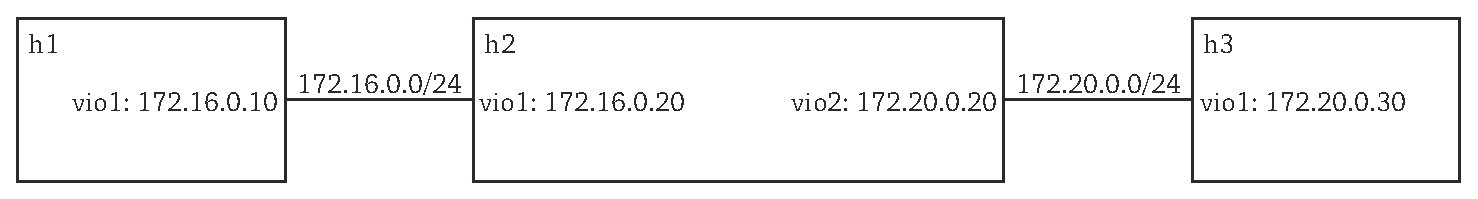
\includegraphics[width=15cm,pagebox=artbox]{figs/quiz01.pdf}
    \caption{問題1:3ノードの単純なネットワークのトポロジ図} \label{fig:quiz01}
\end{figure}

\subsubsection{4ノードのネットワーク}

図~\ref{fig:quiz02}のようなネットワークがあるとする。
このとき、各ノードから全てのノードへIPv4パケットが到達するように、
ノードh1〜h4を設定せよ。

\begin{figure}
    \centering
    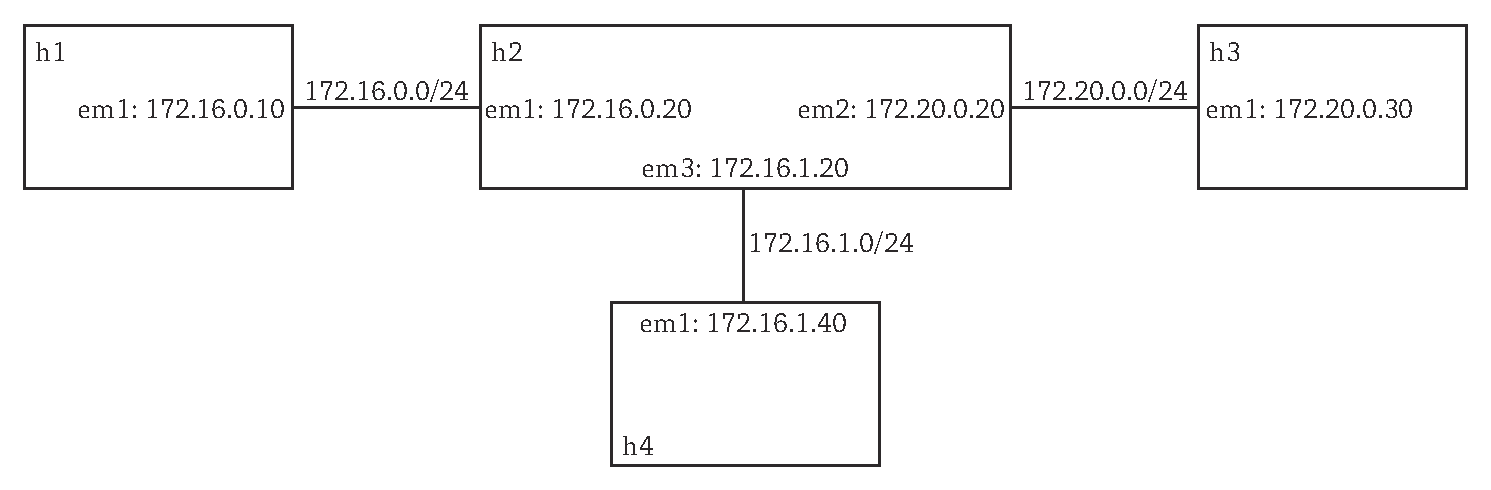
\includegraphics[width=15cm,pagebox=artbox]{figs/quiz02.pdf}
    \caption{問題1:4ノードネットワークのトポロジ図} \label{fig:quiz02}
\end{figure}

\subsection{パケットフィルタ}

\subsubsection{DMZ(DeMilitarized Zone)}


\subsection{VLAN}

\subsection{NAT}

\subsection{ブリッジ}